\subsection{AD9850}

AD9850 je integrisano kolo firme Analog Devices i koristi \gls{dds} tehnologiju
zajedno sa \gls{dac} i brzim komparatorom generiše precizan sinusni i
pravougaoni signal programabilne frekvencije visoke preciznosti. \\
Pravougaoni signal je generisan pomoću sinusne funkcije i komparatora.
Vreme ispune pravougaone funkcije se podešava analognim ulazom na komparatoru,
pa nije moguće digitalno podešavanje bez eksternih komponenti. \\

\begin{figure}[H]
  \centering{
    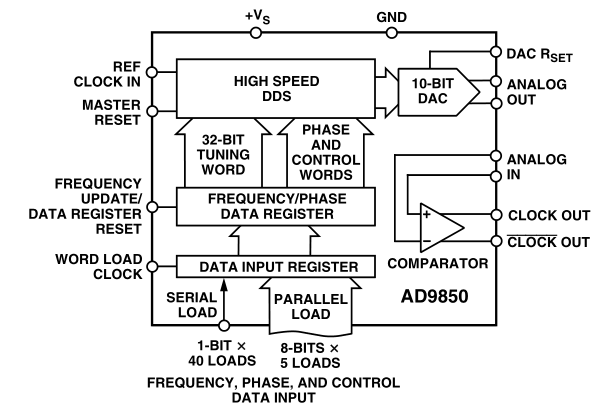
\includegraphics[width=10cm]{img/AD9850_bd.png}
  \caption{Funkcionalni dijagram AD9850\cite{AD9850_ds}}
  \label{func_bd_ad9850}
}
\end{figure}

Frekvencija se podešava postavljanjem 32-bitnog registra na željenu vrednost,
ovime je postignuta preciznost od 0.0291 Hz pri frekvenciji referentnog oscilatora od 125
MHz. \\
\gls{dds} omogućava frekvenciju do polovine referentnog takta, ali je \gls{dac}
ograničava na 40 MHz.
Pored podešavanja frekvencije moguće je i podešavanje faze između dva analogna
izlaza. \\

Moguća je promena izlazne frekvencije brzinom do 23 miliona
novih frekvencija u sekundi.
Ova brzina će zavisiti od načina upisivanja u konfiguracioni registar.
Moguće je upisivati konfiguraciju serijski ili 8-bita paralelno.
U slučaju serijskog upisa potrebno je upisati 40-bita što će oduzeti 40 upisnih
taktova, prilikom paralelnog upisa potrebno je 5 upisnih taktova. \\

\subsubsection{Reset sekvenca}
Pre učitavanja konfiguracionog registra potrebno je resetovati AD9850.
Kako bi se AD9850 resetovao potrebno je generisati sekvencu kao na slici(\ref{ad9850_rst_seq}). \\

\begin{figure}[H]
  \centering{
    \scalebox{1.2}{
      \\
\begin{tikztimingtable}[%
  timing/dslope=0.1,
  timing/.style={x=5ex,y=2ex},
  x=5ex,
  timing/rowdist=4ex,
  timing/name/.style={font=\sffamily\scriptsize}
  ]
  \busref{RST}      & 1u 1L 1H 4L U \\
  \busref{W\_CLK}   & 1u 2.5L 1H 2.5L U \\
  \busref{FQ\_UD}   & 1u 4.0L 1H 1.0L U \\
  \busref{DATA}     & 4U 1L 2.5L  \\
  \extracode
  \begin{pgfonlayer}{background}
  \end{pgfonlayer}
\end{tikztimingtable}
    }}
  \caption{Reset sekvenca}
  \label{ad9850_rst_seq}
\end{figure}

Nakon resetovanja AD9850 je spreman za prihvatanje konfiguracije i generisanje signala.
Reset sekvencu neophodno je generisati prilikom uspostavljanja napajanja, dok prilikom promene
konfiguracije reset nije neophodno odraditi.

\subsubsection{Konfiguracioni registar}

AD9850 se u potpunosti upravlja preko jednog 40-bitnog registra kojim se
podešava frekvencija signala, faza i kontrolni bitovi.

\begin{register}{H}{Konfiguracioni registar}{}% name=example
  \label{example}%
  \regfield{Freq B4}{8}{32}{{Freq b31-b24}}%
  \regfield{Freq B3}{8}{24}{{Freq b23-b16}}%
  \regfield{Freq B2}{8}{16}{{Freq b15-b8}}%
  \regfield{Freq B1}{8}{8}{{Freq b7-b0}}%
  \regfield{Phase}{5}{3}{{Phase b4-b0}}%
  \regfield{Power}{1}{2}{{PD}}%
  \regfield{Control}{2}{0}{{Control}} \\
  \begin{regdesc}\begin{reglist}[Request~Depth]
    \item [Freq B4-B1] Podešava izlaznu frekvenciju generatora.\\
      Vrednost ovog registra može se dobiti sledećom formulom:
      \[
      Freq [31:0] = \frac{freq*2^3^2}{DDS\_CLK}
      \] \\
      freq je željena frekvencija, DDS\_CLK je referentni takt.
    \item [Phase] Podešava fazu.
    \item [Power] Kada je ovaj bit setovan na jedinicu AD9850 je u Power-Down modu.
    \item [Control] Treba biti 0 kako bi oba \gls{dac} izlaza bila aktivna.
    \end{reglist}\end{regdesc}
\end{register}

\subsubsection{Sekvenca za učitavanje konfiguracije}

Nakon uspešnog resetovanja potrebno je upisati željenu konfiguraciju.
Upisivanje u serijskom modu je prikazano na slici (\ref{ad9850_load_seq}).

\begin{figure}[H]
  \centering{
    \scalebox{1.1}{
      \\
\newcommand{\strobeSig}{0.25L 0.5H 0.25L}
\begin{tikztimingtable}[%
  timing/dslope=0.1,
  timing/.style={x=5ex,y=2ex},
  x=5ex,
  timing/rowdist=4ex,
  timing/name/.style={font=\sffamily\scriptsize}
  ]
  \busref{RST}      & 1u 12L \\
  \busref{DATA}     & 1u 1L 1D{Freq b0} 1D{Freq b1} ;[dotted]1D{b2-30}; 1D{Freq b31} 1D{Ctrl b0}
  1D{Ctrl b1} 1D{Power} 1D{Ph b0} ;[dotted]1D{b1-3}; 1D{Ph b4} 1L \\
  \busref{W\_CLK}   & 1u 1L \strobeSig \strobeSig ;[dotted]1L; \strobeSig
  \strobeSig \strobeSig \strobeSig \strobeSig ;[dotted]1L; \strobeSig L \\
  \busref{FQ\_UD}   & 1u 11L \strobeSig \\
  \extracode
  \begin{pgfonlayer}{background}
  \end{pgfonlayer}
\end{tikztimingtable}
    }}
  \caption{Sekvenca serijskog učitavanja}
  \label{ad9850_load_seq}
\end{figure}

Za detaljne informacije o tajminzima pogledati datasheet \cite{AD9850_ds}.

\newpage

\subsubsection{AD9850 modul}

Na slici \ref{ad9850_mod_pinout} prikazan je raspored pinova AD9850 modula
korišćenog u ovom projektu. \\

\begin{figure}[H]
  \centering{
    \includegraphics[width=10cm]{img/AD9850_module.jpg}
    \caption{Raspored pinova AD9850 modula\cite{AD9850_module_pinout}}
    \label{ad9850_mod_pinout}
  }
\end{figure}


Pinove označene sa prefiksom Serial je potrebno koristiti u slučaju serijske
komunikacije. \\
Pinovi obeleženi sa DX se koriste za paralelno upisivanje i u ovom slučaju mogu
se ostaviti nepovezani. \\
Plavom strelicom su označeni izlazni pinovi, od kojih su dva za pravougani
signal dva za sinusni. \\

Na ploči se nalazi referentni oscilator od 125 MHz. \\

Na ulaz internog komparatora za generisanje pravougaonog signala je doveden
napon sa potenciometra na slici, ovo omogućava ručno podešavanje vremena ispune
pravougaonog signala.
Na žalost ovaj modul ne dozvoljava programabilno podešavanje vremena ispune
pravougaonog signala. \\